Para podermos explicar o conceito de \textit{Platooning/Multilane Platooning} em mais profundidade, bem como explicar algumas das abordagens existentes (no mundo real e na literatura) necessitamos introduzir alguns conceitos chave, transversais a quase todas as abordagens. Possíveis conceitos específicos encontrados serão introduzidos na abordagem referente.

\subsection{Controlo lateral}
É considerado que um veículo pode ser \textbf{controlado lateralmente} se a sua direcção (controlo do volante) estiver a cargo do condutor. Neste tipo de controlo a velocidade do veículo estará a cargo do sistema, sendo assim um sistema de condução semi autónoma.

É considerado que um condutor de um  veículo tem apenas \textbf{controlo lateral} sobre o mesmo se apenas a sua interação sobre o volante/direção do veículo tem impacto na condução do mesmo. 
\begin{figure}[H]
    \centering
    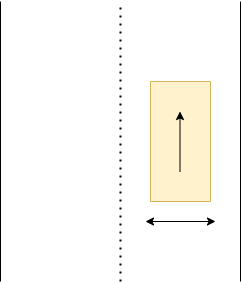
\includegraphics[scale=0.4]{LEI - Article/Images/distLateral.png}
    \caption{Controlo lateral}
    \label{fig:my_label}
\end{figure}

\subsection{Controlo longitudinal}
O conceito de \textbf{controlo longitudinal} é complementar ao conceito de controlo lateral. É considerado que um veículo pode ser controlado longitudinalmente se o controlo da velocidade do mesmo estiver a cargo do condutor.

Um veículo que permita ao condutor ceder o \textbf{controlo lateral} e \textbf{longitudinal} ao sistema pode ser considerado um veículo autónomo.
\begin{figure}[H]
    \centering
    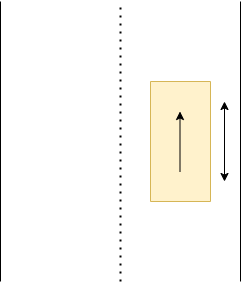
\includegraphics[scale=0.4]{LEI - Article/Images/distLong.png}
    \caption{Controlo longitudinal}
    \label{fig:my_label}
\end{figure}

\subsection{Configuração de um pelotão}
\begin{figure}[H]
    \centering
    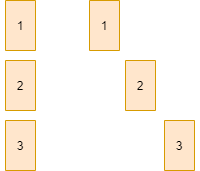
\includegraphics[scale=0.4]{LEI - Article/Images/configPlat.png}
    \caption{Configuração de um pelotão}
    \label{fig:my_label}
\end{figure}
aaaaaaaaaaa\\aaaaaaaaaaa

\subsection{Liderança centralizada}
No controlo de pelotões existe sempre um papel de liderança a ser desempenhado. Com uma \textbf{liderança centralizada} o controlo sobre os integrantes do pelotão encontra-se a cargo de um dos veículos integrantes do mesmo,

sendo que este veículo \textit{"líder"} poderá ser desprovido de certos aspectos de condução autónoma.
\begin{figure}[H]
    \centering
    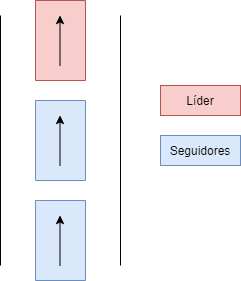
\includegraphics[scale=0.4]{LEI - Article/Images/lidCentr.png}
    \caption{Liderança centralizada}
    \label{fig:my_label}
\end{figure}

\subsection{Liderança descentralizada}
Quando é referida uma \textbf{liderança descentralizada} entende-se que o pelotão não tem um líder físico. Ao contrário da liderança centralizada não existe nenhum veículo responsável por liderar os restantes. O controlo encontra-se numa infraestrutura externa, capaz de comunicar e coordenar os veículos que configuram o pelotão.

\subsection{OBU's}
\textbf{OBU's}, ou \textbf{On Board Units}, são, como o próprio nome indica, unidades que se encontram a bordo do veículo. Estas unidades servem diversos propósitos e, dependendo da abordagem que se esteja a analisar pode ter funcionalidades diferentes. No entanto, e de forma geral, esta unidade serve para receber informação dos sensores do veículo, comunicar com veículos próximos ou até comunicar com uma estação de controlo, no caso de termos liderança descentralizada.


OBUs tem acesso direto aos dados do veiculo (direção, posição, velocidade, etc), geralmente estes dados são processados no veículo de modo a tomar decisões locais. É pertinente tomar decisões de \textit{baixo nível} (como por exemplo reagir a um obstáculo, ou uma travagem inesperada) ao nível do veículo, de modo a minimizar o tempo de reacção. Os veículos próximos deverão também ser notificados desta decisão, notificação esta também a cargo da \textbf{OBU}.